\documentclass[a4paper]{article}

%% Language and font encodings
\usepackage[english]{babel}
\usepackage[utf8x]{inputenc}
\usepackage[T1]{fontenc}
\usepackage{comment}
\usepackage{graphicx}
\usepackage{float}
\usepackage{indentfirst}
\graphicspath{ {images/} }

%% Sets page size and margins
\usepackage[a4paper,top=3cm,bottom=2cm,left=3cm,right=3cm,marginparwidth=1.75cm]{geometry}

%% Useful packages
\usepackage{amsmath}
\usepackage{graphicx}
\usepackage[colorinlistoftodos]{todonotes}
\usepackage[colorlinks=true, allcolors=blue]{hyperref}

\title{Storage Disk Analysis}
\author{Taylor Futral, Sabrina Tsui, and Leah Langford\\ 
UCSC Storage Systems Research Center\\ 
tfutral@ucsc.edu, sctsu@ucsc.edu, llangfor@ucsc.edu}

\begin{document}
\maketitle

\section{Topic}
Different Operating Systems have different access patterns and ways of dealing with the disk drive. The disk drive is a type of storage disk that is used to store data as explained in the background. The goal of this project is to use different types of forensics software to observe where each File System writes to the free list on a disk.\\  
\indent The aim of this project is to analyze where (in terms of sectors and offsets) data is written on the free list, and where on disk that is. By looking at the physical locations in memory things are being written to, we hope to find places in the free list where files can potentially be hidden without being overwritten. The systems that this analysis will focus on are the FreeBSD operating system, the FAT file system (most likely within Linux OS), and the EXT2 file system (also can be found within a Linux OS). Each of these should reveal different patterns of accesses and hopefully will allow us to interpret which file system would be the best for hiding information in the free list.\\
\indent To make this analysis we will be using Sleuth Kit which is a library that exists within Unix and Windows systems that allow for forensic analysis of computer systems. It is capable of parsing all the file systems that we are interested including EXT2, FAT and UFS. Assuming Sleuth Kit works with our hardware and virtual machines, it should be the perfect tool for the job. We plan to use VirtualBox as our virtual machine to host the operating systems containing the file systems of interest. This means that the parameters and settings for one set-up should match the set ups for the other systems too.\\
\indent Our intention with this project is not only to learn where and how each operating system is writing to in the free list but also to learn more about the disk and file systems in general. This learning opportunity should be significantly helpful to improving our knowledge and command as computer science students.

\section{Background}
Storage Disks are mechanisms dedicated to storing data via electrical, optimal, magnetic, and mechanical manipulations to the disk itself. It is rotated in order to store said data in different segments of the disk. For the case of digital disk drives in the use of FAT file systems, the disk is partitioned into multiple “blocks” or clusters (as seen in Figure 1). 

\begin{figure}[H]
\caption{Image of disk partitioned into blocks}
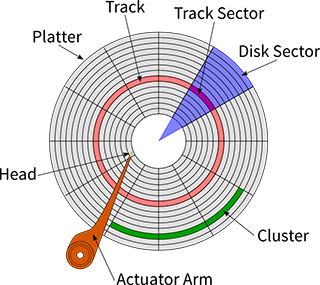
\includegraphics[scale=0.7]{hard-disk-structure}
\end{figure}

\begin{comment}
\begin{figure}
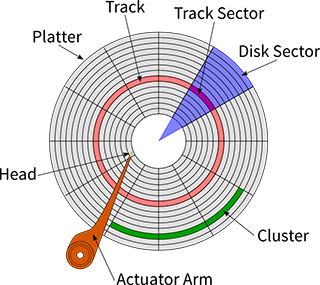
\includegraphics[width=0.3\textwidth]{hard-disk-structure.png}
\caption{\label{fig:hard disk}Disk partitioned into blocks or "clusters".}
\end{figure}
\end{comment}


A free list is a data structure that allows for dynamic memory allocation. Typically this is created and maintained by having each node in a free list point to the next however sometimes the term “free list” is used inappropriately and refers to free memory in general. The significance of the free list for this project is that the different file system’s patterns of accessing it will be observed.\\


Common types of file systems:
\begin{itemize}
\item EXT2 (has bit map, where 1 represents a write, and 0 represents a free spot in memory)
\item NTSF
\item ZFS
\item UFS (contained on versions of FreeBSD)
\item FAT file (contained on versions of Linux)
\item HFS+ / APFS 
\end{itemize}


Sleuth Kit is an open source forensic analysis command line tool. Sleuth Kit can be used to determine operations and accesses within a file system. This functionality can be used to observe where in the free list and on the disk that memory is being written to. 

\section{Procedure}
\subsection{Part 1}
\begin{enumerate}
\item Write test files to memory and find where the data is written to on the disk and free list on these operating systems:\\
\begin{itemize}
\item FreeBSD → UFS/ZFS
\item Linux → FAT file system
\item Linux → EXT2
\end{itemize}
\item Find patterns of where things are written (understand where the computer “decides” to write things).
\item Find spots in the free list where writing there would not be likely to overwrite original data.
\end{enumerate}
\subsection{Part 2}
\begin{enumerate}
\item Compare where the data is written with those operating systems
\begin{itemize}
\item Are there spots in the free list that are common to both file systems?
\end{itemize}
\end{enumerate}

\section{Schedule}
\textbf{\underline{Winter Quarter}}\\
Week 1: Read Disk Tape and Storage Analysis Cost Models, Steganalysis, IEEE Xplore\\
Week 2: Read Usenix paper\\
Week 3: Read up on Sleuth kit and test it\\
Week 4: Read Hard Drive Clusters and File Allocation\\
Week 5: Read up on Ext2 and FreeBSD\\
Week 7: Set up environment and design test cases\\
Week 8: Run the test on the disk where the OS is writing for FreeBSD\\
Week 9: Read up on NTSF, HFS+ / APFS and FAT file system\\
Week 10: Read section 1.3 and 3.2 of Modern Operating Systems\\

\textbf{\underline{Spring Quarter}}\\
Week 1: Read section 3.4, 3.5.8 and 3.5.9 of Modern Operating Systems\\
Week 2: Read section 4.1 Files of Modern Operating Systems\\
Week 3: Read section 4.3.7 and 4.4 of MOS\\
Week 4: Run and the collect data from the FAT file system writes\\
Week 5: Read section 5.5 of MOS and analyze data from FAT file system test\\
Week 6: Run the test on the disk where the OS is writing for Linux’s EXT2 file system\\
Week 7: Analyze and record the data from the Linux EXT2 file system writes\\
Week 8: Draw conclusions and start write up from tests\\
Week 9: Compile and write results in a presentation, paper or poster format\\
Week 10: Edit and revise writing\\

\begin{comment}
\subsection{How to add Comments}

To reply to a comment, simply click the reply button in the lower right corner of the comment, and you can close them when you're done.

Comments can also be added to the margins of the compiled PDF using the todo command\todo{Here's a comment in the margin!}, as shown in the example on the right. You can also add inline comments:

\todo[inline, color=green!40]{This is an inline comment.}

\subsection{How to add Tables}

Use the table and tabular commands for basic tables --- see Table~\ref{tab:widgets}, for example. 

\begin{table}
\centering
\begin{tabular}{l|r}
Item & Quantity \\\hline
Widgets & 42 \\
Gadgets & 13
\end{tabular}
\caption{\label{tab:widgets}An example table.}
\end{table}

\subsection{How to write Mathematics}

\LaTeX{} is great at typesetting mathematics. Let $X_1, X_2, \ldots, X_n$ be a sequence of independent and identically distributed random variables with $\text{E}[X_i] = \mu$ and $\text{Var}[X_i] = \sigma^2 < \infty$, and let
\[S_n = \frac{X_1 + X_2 + \cdots + X_n}{n}
      = \frac{1}{n}\sum_{i}^{n} X_i\]
denote their mean. Then as $n$ approaches infinity, the random variables $\sqrt{n}(S_n - \mu)$ converge in distribution to a normal $\mathcal{N}(0, \sigma^2)$.


\subsection{How to create Sections and Subsections}

Use section and subsections to organize your document. Simply use the section and subsection buttons in the toolbar to create them, and we'll handle all the formatting and numbering automatically.

\subsection{How to add Lists}

You can make lists with automatic numbering \dots

\begin{enumerate}
\item Like this,
\item and like this.
\end{enumerate}
\dots or bullet points \dots
\begin{itemize}
\item Like this,
\item and like this.
\end{itemize}

\subsection{How to add Citations and a References List}

You can upload a \verb|.bib| file containing your BibTeX entries, created with JabRef; or import your \href{https://www.overleaf.com/blog/184}{Mendeley}, CiteULike or Zotero library as a \verb|.bib| file. You can then cite entries from it, like this: \cite{greenwade93}. Just remember to specify a bibliography style, as well as the filename of the \verb|.bib|.

You can find a \href{https://www.overleaf.com/help/97-how-to-include-a-bibliography-using-bibtex}{video tutorial here} to learn more about BibTeX.

We hope you find Overleaf useful, and please let us know if you have any feedback using the help menu above --- or use the contact form at \url{https://www.overleaf.com/contact}!
\fi%----------------to here---------just incase we need it----------------
\end{comment}
\nocite{*}
\bibliographystyle{alpha}
\bibliography{storage}
\end{document}